\documentclass[
	usepdftitle=false,
	xcolor={table, dvipsnames},
	hyperref={
		pdftitle={Multicast totalmente e causalmente ordinato in Go},
    	pdfauthor={A. Chillotti}
    }
]{beamer}

\mode<presentation> {

% The Beamer class comes with a number of default slide themes
% which change the colors and layouts of slides. Below this is a list
% of all the themes, uncomment each in turn to see what they look like.

%\usetheme{default}
%\usetheme{AnnArbor}
%\usetheme{Antibes}
%\usetheme{Bergen}
\usetheme{Berkeley}
%\usetheme{Berlin}
%\usetheme{Boadilla}
%\usetheme{CambridgeUS}
%\usetheme{Copenhagen}
%\usetheme{Darmstadt}
%\usetheme{Dresden}
%\usetheme{Frankfurt}
%\usetheme{Goettingen}
%\usetheme{Hannover}
%\usetheme{Ilmenau}
%\usetheme{JuanLesPins}
%\usetheme{Luebeck}
%\usetheme{Madrid}
%\usetheme{Malmoe}
%\usetheme{Marburg}
%\usetheme{Montpellier}
%\usetheme{PaloAlto}
%\usetheme{Pittsburgh}
%\usetheme{Rochester}
%\usetheme{Singapore}
%\usetheme{Szeged}
%\usetheme{Warsaw}

% As well as themes, the Beamer class has a number of color themes
% for any slide theme. Uncomment each of these in turn to see how it
% changes the colors of your current slide theme.

%\usecolortheme{albatross}
%\usecolortheme{beaver}
%\usecolortheme{beetle}
%\usecolortheme{crane}
%\usecolortheme{dolphin}
%\usecolortheme{dove}
%\usecolortheme{fly}
%\usecolortheme{lily}
%\usecolortheme{orchid}
%\usecolortheme{rose}
%\usecolortheme{seagull}
%\usecolortheme{seahorse}
%\usecolortheme{whale}
%\usecolortheme{wolverine}

%\setbeamertemplate{footline} % To remove the footer line in all slides uncomment this line
%\setbeamertemplate{footline}[page number] % To replace the footer line in all slides with a simple slide count uncomment this line

%\setbeamertemplate{navigation symbols}{} % To remove the navigation symbols from the bottom of all slides uncomment this line
}

\usepackage[utf8]{inputenc}
\usepackage[italian]{babel}
\usepackage[T1]{fontenc}
\usepackage{graphicx}
\usepackage{booktabs}
\usepackage{subcaption}
\usepackage{accents}
\usepackage{adjustbox}

\setlength{\arrayrulewidth}{0.1em}
\renewcommand{\arraystretch}{1.2}

\title[Progetto SDCC]{Multicast totalmente e causalmente ordinato in Go} 

\author{A. Chillotti}

\institute[]{Università degli studi di Roma Tor Vergata}
\date{11 Novembre 2021}

\usefonttheme[onlymath]{serif}
\graphicspath{ {./figs/} }
\definecolor{code_purple}{rgb}{0.5,0,0.35}

\begin{document}

\begin{frame}
\titlepage
\end{frame}

\begin{frame}
\frametitle{Indice}
\tableofcontents
\end{frame}

\section{Servizi richiesti} 
\begin{frame}
\frametitle{Presentazione del caso di studio}
\begin{block}{Servizi richiesti}
\begin{itemize}
\item Un servizio di registrazione dei processi che partecipano al gruppo di comunicazione multicast.
\item Il supporto dei seguenti algoritmi di multicast:
\begin{enumerate}
\item Multicast totalmente ordinato implementato in modo centralizzato tramite un sequencer;
\item Multicast totalmente ordinato implementato in modo decentralizzato tramite l’uso di clock logici scalari;
\item Multicast causalmente ordinato implementato in modo decentralizzato tramite l’uso di clock logici vettoriali.
\end{enumerate}
\end{itemize}
\end{block}
\end{frame}

\section{Assunzioni}
\begin{frame}
\frametitle{Assunzioni}
Le assunzioni che sono state fatte per realizzare questo applicativo sono:
\begin{itemize}
\item Comunicazione affidabile
\item Comunicazione \textit{FIFO} ordered
\item Ritardo massimo nell'invio del messaggio pari a $3$ secondi
\end{itemize}
\end{frame}

\section{Scelte progettuali}
\begin{frame}
\frametitle{Consegna su file}
\begin{block}{File di consegna}
È stato scelto di simulare la consegna di un messaggio attraverso il salvataggio su un file poiché ritenuto semplice ed elegante. Inoltre, questa scelta ha permesso di utilizzare questo file come log del sistema.

\begin{table}[ht!]
  \label{tab:file}
   \begin{adjustbox}{max width=0.5\textwidth}
  \begin{tabular}{ccccl}
    \toprule
    \textit{Id} & \textit{Timestamp} & \textit{Username} & \textit{Messaggio} \\
    \midrule
    1 & 12:59:32 & peer\_1 & messaggio 1 \\
    2 & 13:02:17 & peer\_2 & messaggio 2 \\
    3 & 13:05:27 & peer\_3 & messaggio 3 \\
    4 & 13:08:17 & peer\_2 & messaggio 4 \\
  \bottomrule
\end{tabular}
\end{adjustbox}
\end{table}

\end{block}
\end{frame}

\begin{frame}
\frametitle{Architetture adottate}

\begin{figure}[ht!]
\centering
     \begin{subfigure}[ht]{0.4\textwidth}
         \centering
         \frame{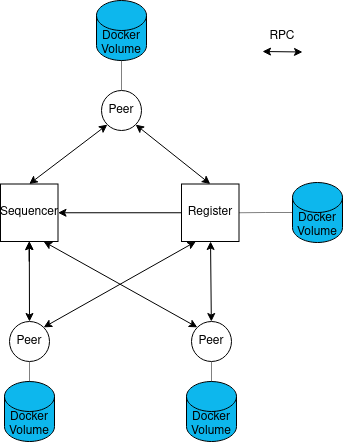
\includegraphics[width=\textwidth]{figs/architecture_1}}
         \caption{Algoritmo 1}
         \label{fig:arch-1}
     \end{subfigure}
     \hfill
     \begin{subfigure}[ht]{0.4\textwidth}
         \centering
         \frame{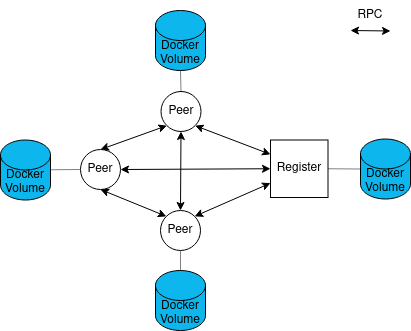
\includegraphics[width=\textwidth]{figs/architecture_2_3}}
         \caption{Algoritmi 2 e 3}
         \label{fig:arch-2-3}
     \end{subfigure}
\end{figure}

\end{frame}

\section{Dettagli generali}
\begin{frame}{Gestione dell'infrastruttura (1)}

\begin{block}{Istanziazione dei container}
È stato utilizzato \textit{Docker} e l'immagine di base selezionata è \texttt{golang:1.16-alpine}.
\end{block}

\begin{block}{Orchestrazione dei container}
È stato utilizzato \textit{Docker Compose}.
\begin{itemize}
\item È stata creata una rete virtuale.
\item È stato creato un profilo \texttt{sequencer}.
\item Sono state create delle variabili d'ambiente che permettono di avere dei parametri configurabili.
\end{itemize}
\end{block}

\end{frame}

\begin{frame}{Gestione dell'infrastruttura (2)}

\begin{block}{Struttura di un peer}
\begin{itemize}
\item È stata implementata una classe \texttt{Peer} che astrae e cattura le caratteristiche e le funzioni di base di un semplice peer.
\item Per gli altri "tipi" di peer sono state realizzate altre classi che vanno ad estendere la classe \texttt{Peer}.
\item Questo approccio ha permesso di avere un codice modulare poiché, nella fase di startup, è presente uno \texttt{switch} che, in base all'algoritmo selezionato, crea le corrette istanze dei peer.
\end{itemize}
\end{block}

\end{frame}

\section{Interazione fra i peer}

\begin{frame}{Comunicazione fra i peer (1)}

\begin{block}{Framework utilizzato}
\begin{itemize}
\item Il meccanismo utilizzato è \textit{Remote Procedure Call}
\item Per l'implementazione di RPC è stato usato il package \texttt{"net/rpc"}
\end{itemize}
\end{block}

\begin{block}{Registrazione al gruppo multicast}
I peer si devono registrare per scambiare delle informazioni (i.e. indirizzo ip, username, numero di porta) con il nodo \texttt{register}. Quest'ultimo ha il compito di inviare queste informazioni:
\begin{itemize}
\item A tutti i nodi registrati
\item Al \texttt{Sequencer}, se selezionato l'algoritmo 1
\end{itemize}
\end{block}
\end{frame}

\begin{frame}{Comunicazione fra i peer (2)}

\begin{block}{Struttura \texttt{Packet}}
Per la comunicazione e lo scambio di messaggi fra i vari peer è stata astratta la figura del pacchetto, ovvero è stata definita la seguente struttura dati.
\begin{figure}[ht]
\centering
\frame{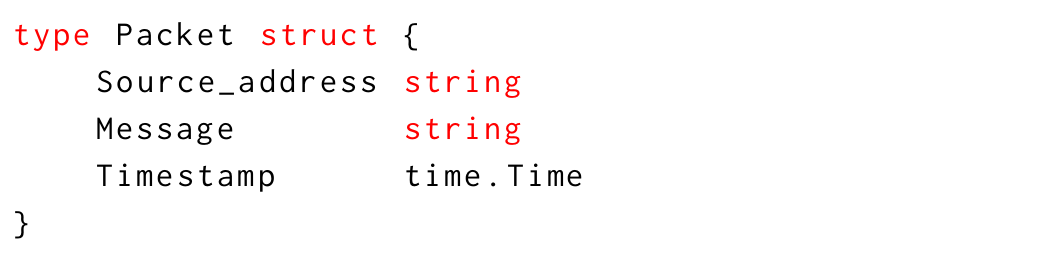
\includegraphics[width=0.6\textwidth]{figs/packet}}
\end{figure}
\end{block}

\begin{block}{Gestione delle connessioni}
È stato implementato un meccanismo di timeout. In particolare, si è scelto che, se all'interno del gruppo multicast ci sono $N$ peer, allora un peer prima di chiudere le connessioni e l'applicazione attenderà $10 \cdot N$ secondi.
\end{block}

\end{frame}

\section{Algoritmi}

\begin{frame}{Descrizione degli algoritmi (1)}

\begin{block}{Algoritmo 1}
In fase di invio di un messaggio, il peer mittente prepara il \texttt{Packet} ed invia il messaggio al nodo \textit{Sequencer}. A sua volta, il \textit{Sequencer} targa il messaggio con un Id.

L'idea addottata, per quanto riguarda un nodo ricevente, è la seguente:
\begin{enumerate}
\item Alla ricezione, il messaggio viene posto all'interno di un buffer (\texttt{channel})
\item In fase di consegna, viene scannerizzato ciclicamente il buffer finché non è presente il messaggio da inviare al livello applicativo.
\end{enumerate}
\end{block}

\end{frame}

\begin{frame}{Descrizione degli algoritmi (2)}

\begin{block}{Algoritmo 2}
\begin{itemize}
\item Per realizzare la lista d'attesa dei messaggi di update ordinati in base al timestamp si è scelto di realizzare una lista collegata
\item L'inserimento in questa lista avviene in maniera ordinata ed ogni suo elemento è la seguente struttura
\begin{figure}[ht]
\centering
\frame{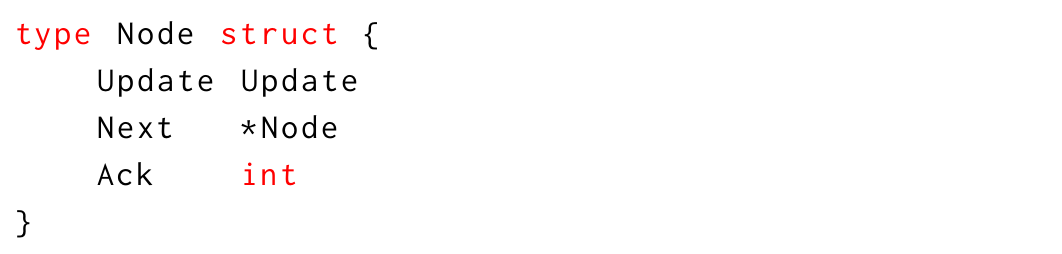
\includegraphics[width=0.6\textwidth]{figs/node}}
\end{figure}
\item Si può notare come l'\texttt{Ack} sia stato inserito come metadato del nodo, in modo tale da facilitare la gestione e l'implementazione della consegna dei pacchetti.
\end{itemize}
\end{block}

\end{frame}

\begin{frame}{Descrizione degli algoritmi (3)}

\begin{block}{Algoritmo 3}
\begin{itemize}
\item Si è nuovamente fatto uso di un buffer per la memorizzazione dei pacchetti ricevuti
\item È stata creata la classe \texttt{Vector Clock} per astrarre il concetto di clock vettoriale e definire alcuni metodi base per la sua gestione
\item L'idea adottata per la ricezione e la consegna è similare a quanto descritto per gli algoritmi precedenti
\end{itemize} 
\end{block}

\end{frame}

\section{Piattaforma software}
\begin{frame}{Piattaforma software}

\begin{block}{Software}
\begin{itemize}
\item Ubuntu 20.04.3 LTS
\item \textit{Go}
\item \textit{Docker}
\item \textit{Docker Compose}
\end{itemize}
\end{block}

\begin{block}{Frontend}
Le librerie utilizzate sono:
\begin{itemize}
\item \texttt{"github.com/docker/docker/api/types"}
\item \texttt{"github.com/docker/docker/client"}
\end{itemize}
\end{block}

\end{frame}

\section{Testing}

\begin{frame}{Test algoritmo 1}

\begin{block}{Un solo sender}
\begin{itemize}
\item Un peer invia sei messaggi, uno dopo l'altro in modo tale da rispettare l'assunzione \textit{FIFO} ordered
\item Il risultato aspettato è che ogni peer consegni, nello stesso identico ordine, i messaggi ricevuti al livello applicativo
\end{itemize}

\end{block}

\begin{block}{Più sender}
\begin{itemize}
\item Ogni peer invia un messaggio al \textit{sequencer} e dopo aver inviato il primo messaggio, ne inoltra un altro
\item Il risultato aspettato è che ogni peer consegni, nello stesso identico ordine, i messaggi ricevuti al livello applicativo
\end{itemize}
\end{block}

\end{frame}

\begin{frame}{Test algoritmo 2}

\begin{block}{Un solo sender}
\begin{itemize}
\item Un peer invia sei messaggi, uno dopo l'altro in modo tale da rispettare l'assunzione \textit{FIFO} ordered
\item Il risultato aspettato è che nessun peer consegni messaggi a livello applicativo, in quanto non viene mai rispettata la condizione di consegna poiché è solamente un peer ad effettuare l'inoltro del messaggio in multicast
\end{itemize}
\end{block}

\begin{block}{Più sender}
\begin{itemize}
\item Ogni peer invia un messaggio al \textit{sequencer} e dopo aver inviato il primo messaggio, ne inoltra un altro
\item Il risultato aspettato è che i primi messaggi consegnati da ciascun peer siano i medesimi
\end{itemize}
\end{block}

\end{frame}

\begin{frame}{Test algoritmo 3}

\begin{block}{Un solo sender}
\begin{itemize}
\item Un peer invia sei messaggi, uno dopo l'altro in modo tale da rispettare l'assunzione \textit{FIFO} ordered
\item Il risultato aspettato è che ogni peer consegni, nello stesso identico ordine
\end{itemize}
\end{block}

\begin{block}{Più sender}
\begin{itemize}
\item Si è seguito uno schema ben preciso

\begin{figure}[ht!]
\centering
\frame{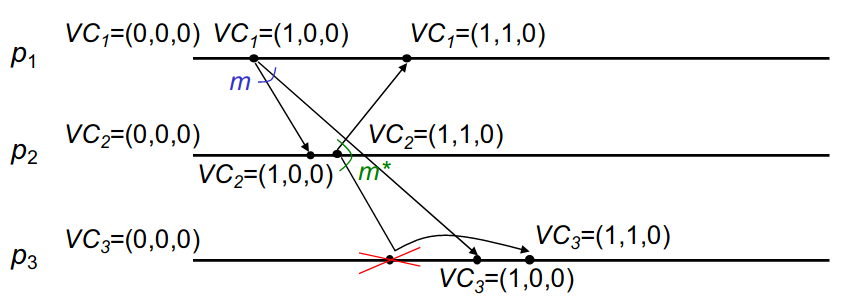
\includegraphics[width=0.4\textwidth]{figs/test}}
\end{figure}
\item Il risultato aspettato è che tutti i peer consegnino i messaggi rispettando la relazione di causa-effetto
\end{itemize}
\end{block}

\end{frame}

\end{document} 